\chapter{Fahrzeugprototyp}
\label{cha:Prototyp}
\section{Vision}
Das Gesamtkonzept für den Fahrzeugprototypen basiert auf der Vision eines \glqq Fahrzeuges als Leinwand\grqq{} (englisch: \glqq Car as a canvas\grqq{}). Das Zielbild dieser Vision ist ein Fahrzeug, das auf vollständiger Weise seine Wahrnehmung auf den Menschen verändern kann. Besonders die visuelle Wahrnehmung ist hier im Vordergrund der Vision, aber diese bleibt nicht singulär, sondern die anderen Wahrnehmungsarten sollen die visuelle Wahrnehmung unterstützen.\\
Unter der übergeordneten Vision das Fahrzeug als Leinwand zu betrachten, bildet das Gesamtkonzept des Prototypen einen möglichen ersten Schritt in Richtung der Vision.
\section{Gesamtkonzept}
Das Gesamtkonzept besteht im Kern um digitale Kunst im Fahrzeug. Kunden können unterschiedliche digitale Kunstinhalte, sogenannte Kollektionen, erwerben und diese Kollektionen in ihrem Fahrzeug aktivieren. Die Kollektionen bestehen aus mehreren inhaltlichen Bestandteilen, welche auf neuartigen und bestehenden Fahrzeugkomponenten im Fahrzeug dargestellt werden. Die Darstellung der Inhalte der Kollektionen kann entweder durchgehend sein oder nur durch bestimmte Trigger wie zum Beispiel das Entriegeln der Türen ausgelöst werden.
Neben optischen Komponenten unterstützen haptische, olfaktorische und akustische Komponenten die Kollektionen. Dazu bilden Augmented Reality (AR\nomenclature{AR}{Augemented Reality}) Anwendungen weitere Darstellungen der Kollektionen mit Hilfe von einer eigenen App auf einem Mobiltelefon.\\
Die App ist für den Besitzer das zentrale Steuersystem in der unterschiedliche Aktionen auf den einzelnen Seiten verfügbar sind:
\begin{itemize}
	\item Kollektionen können auf digitalen Börsen gehandelt werden
	\item Gekaufte Kollektionen können im Fahrzeug aktiviert werden oder durch AR auf dem Mobiltelefon gezeigt werden
	\item zusätzliche AR Inhalte zu den Kollektionen können auf dem Mobiltelefon gezeigt werden
	\item einzelne Komponenten der aktivierten Kollektion können deaktiviert werden
	\item über ein eigenes Profil kann mit anderen Besitzern von Kollektionen Bilder durch ein soziales Netzwerk ausgetauscht werden
\end{itemize}
Im Gegensatz zu bisherigen Individualisierungsmöglichkeiten, wie zum Beispiel Ambientebeleuchtung oder LED Scheinwerfer, können die Kollektionen in diesem Gesamtkonzept zum Einen dynamisch ihre Inhalte verändern und zum Anderen das gesamte Erscheinungsbild des Fahrzeuges durch ganzheitlich verändern. Daneben bietet das Gesamtkonzept ein Ökosystem für den Handeln und die Interaktion für Kollektionen als digitale Wertgegenstände.
\section{Beschreibung}
Der Prototyp wurde unter den Leitlinien des Gesamtkonzeptes entwickelt. Aufbauend auf einem produzierten elektrischen Serienfahrzeug wurden im Exterieur und Interieur Teile ergänzt und teilweise mit anderen Komponenten ausgetauscht, um das Gesamtkonzept zu folgen. Die Serienfunktionen wurden zum größten Teil durch die Umbauten nicht beeinträchtigt.\\
Durch Zeit- und Budgetknappheit besitzt das Fahrzeug nicht alle Ideen des Gesamtkonzeptes. Bei den Hardware Komponenten gibt es keine mit olfaktorischen Sinneseindrücken. Die App besitzt alle oben beschriebenen Funktionen zumindest als Schaubilder, aber hat nur die Auswahl und Steuerung der Kollektionen und AR Inhalte als Funktionen implementiert.
\section{Exterieur Komponenten}
Das Fahrzeug hat sowohl im Exterieur als auch im Interieur Komponenten verbaut. Zuerst werden die Komponenten im Exterieur und dann im Interieur vorgestellt. Die Komponenten wurden nach der verwendeten Technik und dem Ort benannt und nicht nach den Markennamen. Die Einteilung erfolgt nach der Betrachtungsweise innerhalb oder außerhalb des Fahrzeugs der Komponenten. Exterieur Komponenten werden von Beobachtern außerhalb des Fahrzeugs betrachtet. Interieur Komponenten entsprechend von innen.\\
Im Exterieur sind dies ein E-Papier in der Frontschürze, ein durchgehendes LED-Streifen in der Frontschürze, E-Papier Embleme über den beiden vorderen Radkästen, LED-Streifen in allen vier Radkästen, Videoprojektoren in den beiden Außenspiegel, nach außen gerichtete Bildschirme in den hinteren Seitenfenstern, ein LED-Streifen in der Heckleuchte und zwei kleine E-Papiere unterhalb der Heckleuchte.\\
Im folgenden werden alle Exterieur Komponenten nähe betrachtet:
\subsection{E-Papier in der Frontschürze}
Das E-Papier befindet sich hinter einer Scheibe mit einem Markenlogo in der Mitte der Fahrzeugfront und schließt an den Seiten über eine Abmaskierung auf die beiden Frontlichter an. Das E-Papier bewirkt mit der Laminierung an der Scheibe einen räumlichen Effekt, wonach das Markenlogo vor dem E-Papier hervor strahlt.
Auf dem E-Papier werden graphische Designs dargestellt, die Betrachter vor dem Auto sehen können.
\subsection{LED-Streifen in der Frontschürze}
Der LED-Streifen ist dreiteilig aufgeteilt. Die zwei äußeren Teile befinden sich in der Frontleuchten und schließen auf gleicher Höhe mit dem mittleren Streifen an. Der mittlere Streifen befindet sich oberhalb des E-Papier in der Frontschürze.
Auf dem Streifen werden dynamische bunte Lichtsequenzen gezeigt.
Zusammen mit dem E-Papier in der Frontschürze bilden diese zwei Komponenten die Darstellung der Kollektionen im Frontbereich.
\subsection{E-Papier Embleme über den vorderen Radkästen}
Oberhalb der Radkästen befinden sich ca 20 cm Breite und 8 cm hohe E-Papiere. An dieser Stelle befand sich vorher ein Emblem der Fahrzeugbezeichnung.
Die E-Papiere werden genutzt, um den Namen der verwendeten Kollektion anzuzeigen.
\subsection{LED-Streifen in den Radkästen}
In allen vier Radkästen befinden sich LED-Streifen am äußeren Rand und strahlen durch eine Leiste nur in den Radkasten Innenraum auf den oberen Halbkreis des Reifenprofils. 
\subsection{Videoprojektoren in den Außenspiegeln}
In den Außenspiegeln wurde der Innenraum mit der Spiegelmechanik ausgebaut und Videoprojektoren eingebaut. Der nach unten ausgerichtete Videoprojektor bestrahlt die Flächen durch ein Loch an der Unterseite des Außenspiegels vor den vorderen Türen.
Durch den Videoprojektor können Videos auf dem Boden gezeigt werden.
\subsection{Bildschirme in den hinteren Seitenfenstern}
In den hinteren Seitenfenstern befinden sich hinter der unbeweglichen Nebenscheiben, die mit einer Leiste von den beweglichen Hauptglasscheiben getrennt sind, Bildschirme. Diese können von außen betrachtet werden. Die Rückseite der Bildschirme ist von innen mit einer schwarzen Kunststoffverkleidung für die Passagiere abgedeckt.\\
Zusammen mit den LED-Streifen in den Radkästen und den Videoprojektoren in den Außenspiegeln bilden die Bildschirme in den Seitenfenstern die optische Darstellung der Kollektionen im Seitenbereich.
\subsection{LED-Streifen in der Heckleuchte}
In der Serienheckleuchte wurde das rote Leuchtband mit einem LED-Streifen getauscht. Der Streifen ist dreigeteilt mit dem mittleren Teil in der Heckklappe und den zwei äußeren Teilen im hinteren Kotflügel.
\subsection{E-Papier in der Heckleuchte}
Direkt unterhalb der Heckleuchten sind zwei E-Papiere in der Heckklappe eingebaut.
Diese E-Papiere haben eine ähnliche Größe wie die E-Papiere oberhalb der Radkästen und werden auch genutzt, um den Namen der Kollektionen zu zeigen.\\
Zusammen mit dem LED-Streifen in der Heckleuchte bilden die E-Papiere die Heckansicht der Kollektion für Betrachter.
\section{Interieur Komponenten}
Im Interieur sind die Komponenten ein durchgehender LED-Streifen von den hinteren Türen über die vorderen Türen bis über das gesamte Cockpit, in den Türen eine LED Matrizen, Bildschirme in der Einstiegsleiste der vorderen Türen, Videoprojektoren im Fußraum der Frontsitze, Benutzeroberflächen für den Fahrer- und den Zentralbildschirm, eine morphende Oberfläche in der Mittelkonsole, einen durchsichtigen Bildschirm im Dachfenster und eine LED Matrix im Dachhimmel.\\
Daneben sind weitere Komponenten Duftflakons im Innenraum, Bildschirmoberflächen im Cockpit und ein Soundplayer im Innenraum.
Im folgenden werden alle Interieur Komponenten näher vorgestellt.
\subsection{LED-Streifen im Interieur}
Der LED-Streifen ist fünf geteilt und erstreckt sich im oberen Bereich der vier Türverkleidungen und schließt über das Cockpit zu einem einheitlichen Band ab. Der Streifen befindet sich hinter einer Streulichtscheibe, damit der Betrachter nicht die einzelnen LED erkennen kann. 
Der Streifen spielt dynamische Inszenierungen für die Fahrzeuginsassen ab.
\subsection{Matrix LED Türtafeln}
In allen vier Türverkleidungen befinden sich unterhalb des LED-Streifens ein LED Feld hinter einer Abdeckung mit durchsichtigen Sternen. Die Sterne können somit mit unterschiedlichen Farben angestrahlt werden. 
\subsection{Bildschirme in der Einstiegsleiste}
Anstelle einer Edelstahl Abdeckung mit einem Schriftzug befinden sich in den vorderen Türen Bildschirme in der Einstiegsleiste. Die Bildschirme können bei geöffneter Türe Inhalte dem Fahrzeuginsassen und Betrachter Außerhalb des Fahrzeuges darstellen.
\subsection{Videoprojektoren im Fußraum}
Für die vorderen Fußraumböden wurden zwei Videoprojektoren verbaut. Der linke Videoprojektor befindet sich unterhalb der Lenksäule, der rechte unterhalb des Handschuhfachs. Beide Videoprojektoren strahlen den Fußraum an und können dynamisch Inhalte abspielen.
\subsection{Morphende Oberfläche in der Mittelkonsole}
In der Mittelkonsole wurde das Ablagefach und die abgelederte Abdeckung durch eine neuartige Vorrichtung ersetzt, die von innen mit Hilfe von Formteilen auf die Oberflüche drückt und somit von außen optisch und haptisch spürbar ist. In der Vorrichtung befinden sich in einem Revolver drei Formteile mit unterschiedlicher Ausgestaltung.
\subsection{Durchsichtiger Bildschirm im Dachfenster}
An das Dachfenster wurde ein durchsichtiges Bildschirm geklebt, das bei Betrachten von innen Grafiken darstellen kann.
\subsection{LED Matrix im Dachhimmel}
Im Dachhimmel unter der Stoffverkleidung befindet sich eine LED Matrix. Das Feld kann dynamische Farbeffekte erzeugen.
\subsection{Duftflakons im Innenraum}
Im Innenraum befinden sich Duftflakons, die jeweils für eine bestimmte Kollektion erstellt wurden. Es ist kein technischer Aufbau zur automatischen Beduftung des Innenraumes vorhanden.
\subsection{Bildschirmoberflächen im Cockpit}
Das zentrale Kombiinstrument und das digitale Fahrerdisplays haben die Möglichkeit unterschiedliche Bildschirmoberflächen anzuzeigen.
\subsection{Soundplayer im Innenraum}
Das Soundsystem im Innenraum kann extern über den Zentralrechner angesteuert werden und MP3 Dateien abspielen.
\section{Ansteuerung}
Die Ansteuerung der Komponenten erfolgt über einen zentralen Rechner mit Windows Betriebssystem, der sich im Kofferraum des Fahrzeuges befindet und die Informationen für die Komponenten in einem lokalen Verzeichnis gespeichert hat. Die Komponenten sind entweder direkt über Leitungen oder über eine Wireless Local Area Network (WLAN\nomenclature{WLAN}{Wireless Local Area Network}) Schnittstelle mit dem Rechner verbunden.\\
Die Displays und Beamer sind über HDMI (High Definition Multimedia Interface\nomenclature{HDMI}{High Definition Multimedia Interface}) mit dem Computer verbunden. Die Lichtleisten sind über USB (Universal Serial Bus\nomenclature{USB}{Universial Serial Bus}) mit dem Rechner über ein USB Hub verbunden. Die E-Papier Displays werden von Raspberry Pis angesteuert und sind mit dem Rechner über LAN (Local Area Network\nomenclature{LAN}{Local Area Network}) verbunden. Der Dachhimmel wird über WLAN vom Computer aus angesteuert. Die Lautsprecher werden über einen Verstärker und ein USB Audio Interface mit dem Computer verbunden.\\
An dem Computer ist ein Mobiltelefon über WLAN angeschlossen, das mit Hilfe einer App unterschiedliche Inhalte für die Komponenten auswählen kann.\\
Der Computer hat einen Zugriff auf das Bordnetz des Fahrzeug, um einzelne Signale herauslesen zu können. Durch bestimmte Signaländerungen löst der Computer Sequenzen von Inhalten in den Komponenten aus.\\
Die Komponenten des Prototypen sind damit nicht über das Serienbordnetz des Fahrzeug angeschlossen, sondern sind gesamt von diesem abgekoppelt.

\begin{figure}[hbt]
	\centering
	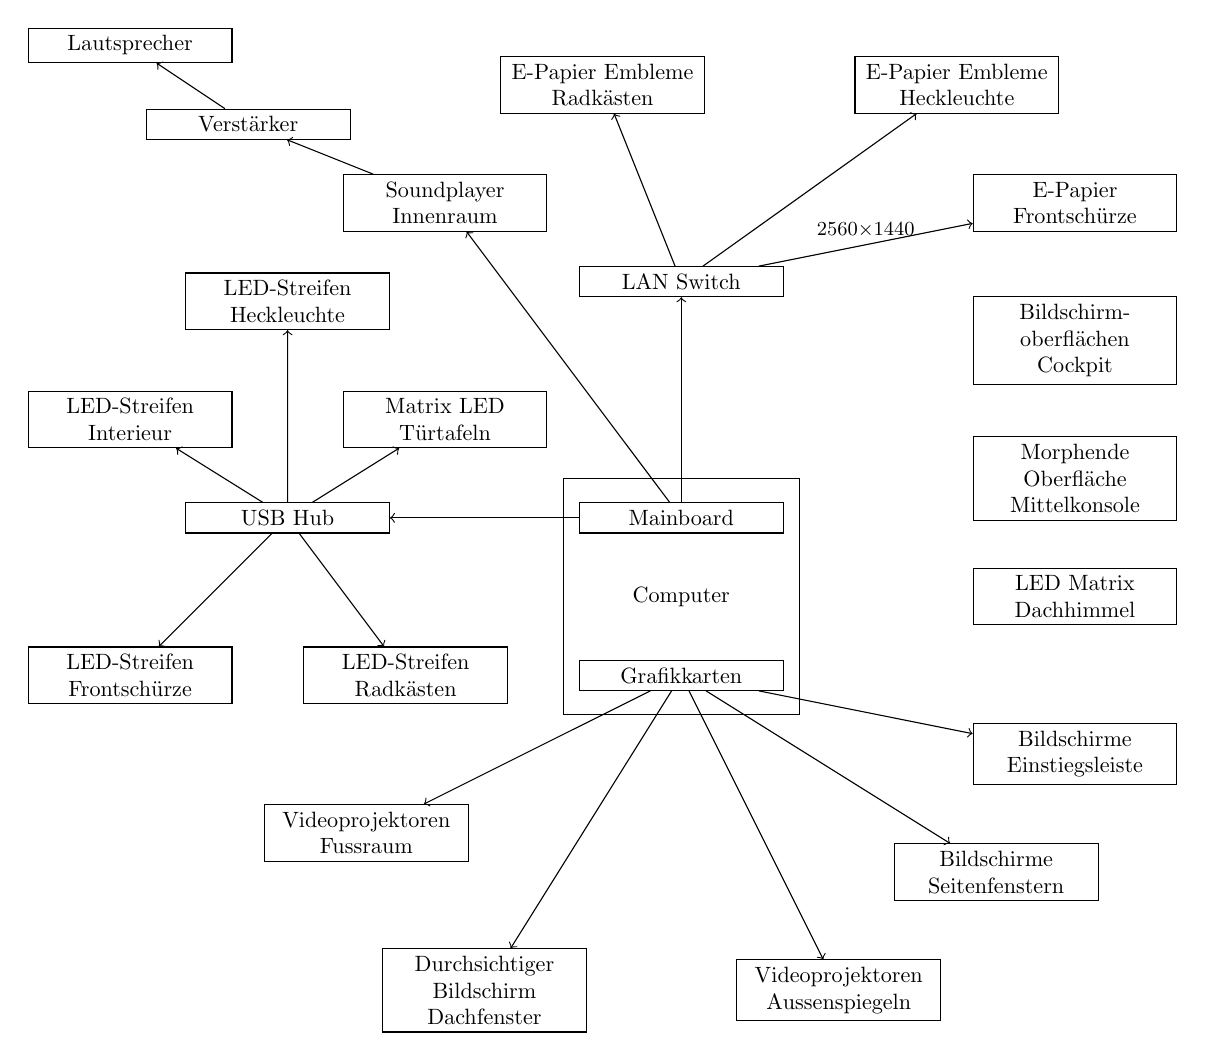
\begin{tikzpicture}[every node/.style={scale=0.8}]
	\node[text width=3.2cm, align=center] (Computer) at (0, -1) {Computer};
	\draw[draw=black] (-1.5,-2.5) rectangle ++(3,3);
	\node[draw, rectangle, text width=3cm, align=center] (Mainboard) at (0, 0) {Mainboard};
	\node[draw, rectangle, text width=3cm, align=center] (Grafikkarten) at (0, -2) {Grafikkarten};
	\node[draw, rectangle, text width=3cm, align=center] (LAN Switch) at (0, 3) {LAN Switch};
	\node[draw, rectangle, text width=3cm, align=center] (E-Papier Frontschürze) at (5, 4) {E-Papier Frontschürze};
	\node[draw, rectangle, text width=3cm, align=center] (LED-Streifen Frontschürze) at (-7, -2) {LED-Streifen Frontschürze};
	\node[draw, rectangle, text width=3cm, align=center] (E-Papier Embleme Radkästen) at (-1, 5.5) {E-Papier Embleme Radkästen};
	\node[draw, rectangle, text width=3cm, align=center] (LED-Streifen Radkästen) at (-3.5, -2) {LED-Streifen Radkästen};
	\node[draw, rectangle, text width=3cm, align=center] (Videoprojektoren Aussenspiegeln) at (2, -6) {Videoprojektoren Aussenspiegeln};
	\node[draw, rectangle, text width=3cm, align=center] (Bildschirme Seitenfenstern) at (4, -4.5) {Bildschirme Seitenfenstern};
	\node[draw, rectangle, text width=3cm, align=center] (LED-Streifen Heckleuchte) at (-5, 2.75) {LED-Streifen Heckleuchte};
	\node[draw, rectangle, text width=3cm, align=center] (E-Papier Embleme Heckleuchte) at (3.5, 5.5) {E-Papier Embleme Heckleuchte};
	\node[draw, rectangle, text width=3cm, align=center] (LED-Streifen Interieur) at (-7, 1.25) {LED-Streifen Interieur};
	\node[draw, rectangle, text width=3cm, align=center] (Matrix LED Türtafeln) at (-3, 1.25) {Matrix LED Türtafeln};
	\node[draw, rectangle, text width=3cm, align=center] (Bildschirme Einstiegsleiste) at (5, -3) {Bildschirme Einstiegsleiste};
	\node[draw, rectangle, text width=3cm, align=center] (Videoprojektoren Fussraum) at (-4, -4) {Videoprojektoren Fussraum};
	\node[draw, rectangle, text width=3cm, align=center] (Morphende Oberfläche Mittelkonsole) at (5, 0.5) {Morphende Oberfläche Mittelkonsole};
	\node[draw, rectangle, text width=3cm, align=center] (Durchsichtiger Bildschirm Dachfenster) at (-2.5, -6) {Durchsichtiger Bildschirm Dachfenster};
	\node[draw, rectangle, text width=3cm, align=center] (LED Matrix Dachhimmel) at (5, -1) {LED Matrix Dachhimmel};
	\node[draw, rectangle, text width=3cm, align=center] (Bildschirmoberflächen Cockpit) at (5, 2.25) {Bildschirm-oberflächen Cockpit};
	\node[draw, rectangle, text width=3cm, align=center] (Soundplayer Innenraum) at (-3, 4) {Soundplayer Innenraum};
	\node[draw, rectangle, text width=3cm, align=center] (USB Hub) at (-5, 0) {USB Hub};
	\node[draw, rectangle, text width=3cm, align=center] (Verstärker) at (-5.5, 5) {Verstärker};
	\node[draw, rectangle, text width=3cm, align=center] (Lautsprecher) at (-7, 6) {Lautsprecher};
	\draw[->] (Mainboard) -> (LAN Switch);
	\draw[->] (Mainboard) -> (Soundplayer Innenraum);
	\draw[->] (Mainboard) -> (USB Hub);
	\draw[->] (Grafikkarten) -> (Bildschirme Seitenfenstern);
	\draw[->] (Grafikkarten) -> (Bildschirme Einstiegsleiste);
	\draw[->] (Grafikkarten) -> (Videoprojektoren Fussraum);
	\draw[->] (Grafikkarten) -> (Videoprojektoren Aussenspiegeln);
	\draw[->] (Grafikkarten) -> (Durchsichtiger Bildschirm Dachfenster);
	\draw[->] (LAN Switch) -> node[above]{\small2560$ \times $1440} (E-Papier Frontschürze);
	\draw[->] (LAN Switch) -> (E-Papier Embleme Radkästen);
	\draw[->] (LAN Switch) -> (E-Papier Embleme Heckleuchte);
	\draw[->] (USB Hub) -> (LED-Streifen Frontschürze);
	\draw[->] (USB Hub) -> (LED-Streifen Radkästen);
	\draw[->] (USB Hub) -> (LED-Streifen Heckleuchte);
	\draw[->] (USB Hub) -> (LED-Streifen Interieur);
	\draw[->] (USB Hub) -> (Matrix LED Türtafeln);
	\draw[->] (Soundplayer Innenraum) -> (Verstärker);
	\draw[->] (Verstärker) -> (Lautsprecher);
\end{tikzpicture}
	\caption[Ansteuerung Komponenten im Prototypen]{Ansteuerung Komponenten im Prototypen}
	\label{fig:tikz_ansteuerung}
\end{figure}